\def\year{2019}\relax
%File: formatting-instruction.tex
\documentclass[letterpaper]{article} %DO NOT CHANGE THIS
\usepackage{aaai19}  %Required
\usepackage{times}  %Required
\usepackage{helvet}  %Required
\usepackage{courier}  %Required
\usepackage{url}  %Required
\usepackage{graphicx}  %Required

%%%%%%%%%%%%%%%%%%%%%
\usepackage[bookmarks=true]{hyperref}
\usepackage{graphicx}
\usepackage[font=footnotesize]{subcaption}
\usepackage[font=footnotesize]{caption}
\usepackage{hyperref}
\usepackage{url}
\usepackage{amsmath,amssymb,amsfonts,amsfonts}
% \usepackage{algorithm}
% \usepackage[noend]{algorithmic}
\usepackage{xspace}
\usepackage{wrapfig}
\usepackage{color}
\usepackage{graphicx}

\usepackage{algorithm}
\usepackage{algorithmicx}
\usepackage[noend]{algpseudocode}
\usepackage{algpseudocode}
\usepackage{parskip}
\usepackage{amsthm}

\algrenewcommand\algorithmicindent{1.0em}%

\newcommand{\calX}{\ensuremath{\mathcal{X}}\xspace}
\newcommand{\calL}{\ensuremath{\mathcal{L}}\xspace}
\newcommand{\calS}{\ensuremath{\mathcal{S}}\xspace}
\newcommand{\calR}{\ensuremath{\mathcal{R}}\xspace}
\newcommand{\calD}{\ensuremath{\mathcal{D}}\xspace}

\newcommand{\sAttract}{\ensuremath{s^{\text{attractor}}_i}\xspace}
\newcommand{\sStart}{\ensuremath{s_{\text{start}}\xspace}}
\newcommand{\sGoal}{\ensuremath{s_{\text{goal}}\xspace}}
\newcommand{\sNom}{\ensuremath{s_{\text{nominal}}\xspace}}

\newtheorem{theorem}{Theorem}
\newtheorem{lemma}{Lemma}
%%%%%%%%%%%%%%%%%%%

\frenchspacing  %Required
\setlength{\pdfpagewidth}{8.5in}  %Required
\setlength{\pdfpageheight}{11in}  %Required
%PDF Info Is Required:
  \pdfinfo{
/Title (Provable Infinite-Horizon Real-Time Planning for Repetitive Tasks)}
\setcounter{secnumdepth}{0}  
 \begin{document}
% The file aaai.sty is the style file for AAAI Press 
% proceedings, working notes, and technical reports.
%
\title{Provable Infinite-Horizon Real-Time Planning for Repetitive Tasks}
\author{
Fahad Islam,
Oren Salzman {\normalfont and}
Maxim Likhachev
\\
The Robotics Institute, Carnegie Mellon University\\
%
\{fi,osalzman\}@andrew.cmu.edu,
maxim@cs.cmu.edu
}
\maketitle

\begin{abstract}
In manufacturing, robots often have to perform highly-repetitive manipulation tasks in structured environments. 
In this work we are interested in the settings where the tasks are similar, yet not identical (e.g., due to uncertain orientation of objects) and motion planning needs to be extremely fast. 
Preprocessing-based approaches prove to be very beneficial in these settings---they analyze the configuration-space offline to generate some auxiliary information which can then be used in the query phase to speedup planning times. 
%
Typically, the tighter the requirement is on query times the larger the memory footprint will be. In particular, for high-dimensional spaces, providing real-time planning capabilities is impractical.
Moreover, as far as we are aware of, none of the general-purpose algorithms come with \emph{provable} guarantees on the real-time performance.
%
To this end, we propose a preprocessing-based method that provides provable bounds on the query time while incurring only a small amount of memory overhead in the query phase.
We evaluate our method on a 7-DOF robot arm and show a speedup of over tenfold in query time when compared to the \textsf{PRM} algorithm, while guaranteeing a maximum query time of less than 4 milliseconds.
\end{abstract}

\section{Introduction}

%1. What is the problem?
Consider the problem of a robot picking up objects from a high-speed conveyor belt and placing them into bins (see Fig.~\ref{fig:PR2}).
Similarly, consider a robot given the task of stock replenishment---moving in a supermarket and loading items from a cart it carries to half-empty shelves.
%2. Why is it relevant?
These problems are examples of repetitive tasks performed by (possibly highly articulated) robots in static environments where the start and goal of each repetitive task is similar, yet not identical, to previous tasks.
Difference in the exact start and goal position may be due to uncertainty in the environment (objects placed on different parts of the conveyor belt or in different orientation) or due to highly-similar tasks (objects placed in similar positions on a shelf).

{\color{blue} I think the motivation is unclear here after reading the first para, and the second para starts kind of out of the blue.}

%3. Why is it hard?
As the set of possible start and goal locations may be large, caching pre-computed paths for all these queries in advance is unmanageable. 
Clearly, once a task is presented to the robot, it can compute a desired path online.
However, this may incur large online planning times that may be unacceptable in many settings.
For example, in our conveyor-belt setting, reducing the planning time immediately corresponds to faster unloading capabilities. 
Moreover, if the planner cannot \emph{guarantee} to pick items from the conveyor in a timely manner, the system is required to account for missed items by e.g., additional conveyor belts that will redirect items back to the robot---a costly backup in terms of both time and space.
Thus, a natural approach is to preprocess the environment in an offline phase to allow for fast planning times online.

%4. What have others done?
One way to preprocess the environment is using the \textsf{PRM} algorithm~\cite{kavraki1996probabilistic}.
Once a a dense roadmap has been pre-computed, any query can be efficiently answered online by connecting the source and goal to the roadmap. 
Query times can be significantly sped up by further preprocessing the roadmaps using landmarks~\cite{paden2017landmark}.
Unfortunately, there is no guarantee that a query can be connected to the roadmap as \textsf{PRM} only provides \emph{asymptotic} guarantees~\cite{KKL98}.
Furthermore, this connecting phase requires running a collision-detection algorithm which is typically considered the computational bottleneck in many motion-planning algorithms~\cite{L06}.

{\color{blue} Cite experience graphs in the context of learning from previous planning episodes. Although the e-graph heuristic speeds up the search but 1. the e-graph heuristic computation itself is expensive 2. the size of e-graph keeps growing and there is no systematic way of maintaing a sparse e-graph.}

Recently, Lehner and  Albu{-}Sch{\"{a}}ffer~\cite{LA18} suggest the repetition roadmap to extend the \textsf{PRM} for the case of multiple highly-similar scenarios.
While their approach exhibits significant speedup in computation time, it still suffers from the previously-mentioned shortcomings.

A complementary approach to aggressively preprocess a given scenario is by minimizing collision-detection time.
However this requires designing robot-specific
circuitry~\cite{MFQSK16}
or limiting the approach to standard manipulators~\cite{YMILV18}.

An alternative approach is to precompute a set of complete paths into a library and given a query, attempt to match complete paths
from the library to the new query~\cite{berenson2012robot,jetchev2013fast}.
Unfortunately, this approach also cannot provide any of the guarantees required by our applications.

Our work bares resemblance to previous work on 
subgoal graphs~\cite{UK17,UK18} and to real-time planning~\cite{KL06,KS09,K90}.
However, in the former, the entire configuration space is preprocessed in order to efficiently answer queries between \emph{any} pair of states which deems it applicable only to low-dimensional spaces.
{\color{blue} Also their $connect$ step is expensive as it requires a Dijkstra's like search to connect to the subgoal graph.} Similarly, in the latter, to provide guarantees on planning time the search only looks at a finite horizon and interleaves planning and execution.

{\color{blue} 
More citations:\\
1. Composition of local potential functions for global robot control and navigation.\\
2. Integrated Planning and Control for Convex-bodied Nonholonomic Systems using Local Feedback Control Policies.

I remember Max mentioning this work once, I haven't read these papers thoroughly though (one of these is a thesis doc). My understanding is that they have a similar idea of constructing these attractions "funnels" which we call subregions. They are using this idea in the controls world while we are doing planning.

3. LQR-Trees: Feedback Motion Planning
on Sparse Randomized Trees \\
This also seems to be a similar idea from the controls community.

These are all well cited papers. You might want to skim through these to get the right context but I think they are relevant.

4. Experience-based planning with sparse roadmap spanners \\
}

\begin{figure}[tb]
  \centering
    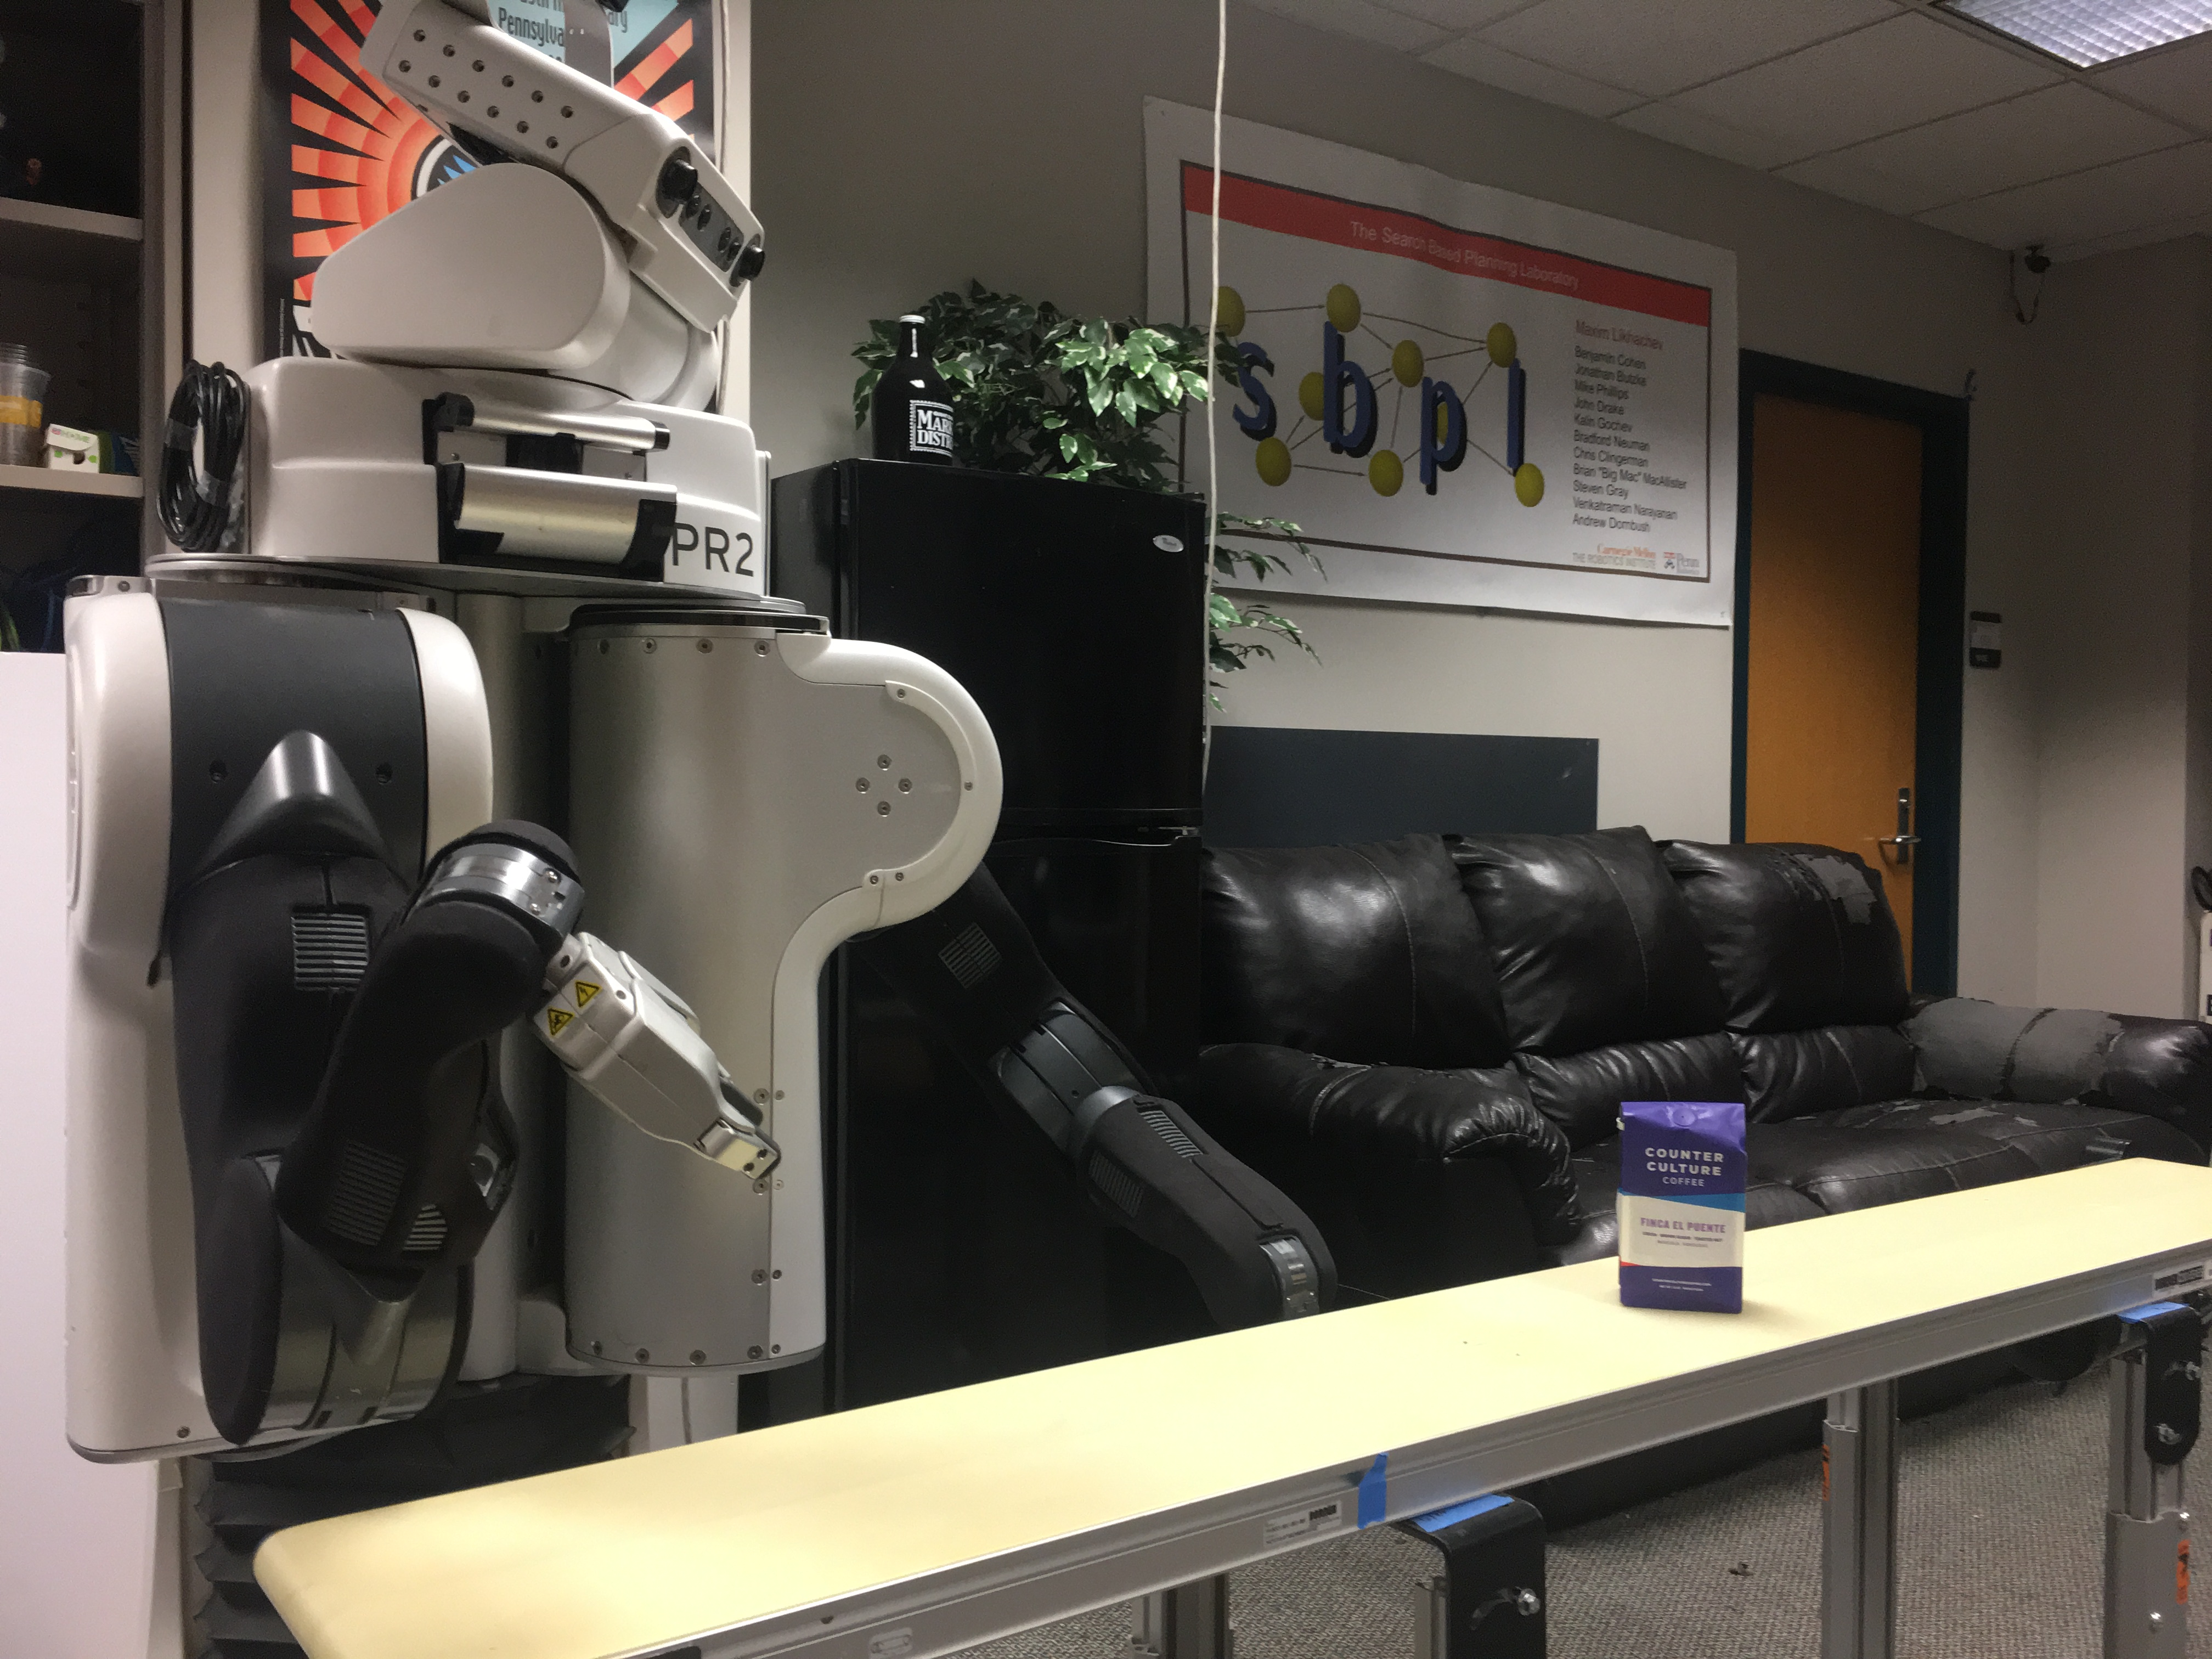
\includegraphics[width=0.25\textwidth]{PR2.jpg}
    % \vspace{-2mm}
  \caption{
  Motivating scenario---a robot (PR2) picking up objects from a conveyor belt.
}
    \label{fig:PR2}
 \vspace{-6mm}
\end{figure}

%5. What's missing?

%6. What is our ONE key insight?
Our key insight is to combine a precomputed library~$\calL$ of paths between \emph{several} start and goal configurations together with a method to connect \emph{any} start and goal configuration to a path in~$\calL$ \emph{without} having to perform collision detection.
This insight allows us to provide \emph{provable bounds} on the time to solve motion-planning queries which is in the order of milliseconds for a seven DOF manipulator.

{\color{blue} We need to redo this para. The workshop reviewer also said that it's unclear}

%7. How do we compare against the state of the art?
We evaluate our approach in simulation on the PR2 robot\footnote{http://www.willowgarage.com/pages/pr2/overview} (see Fig.~\ref{fig:PR2})
and demonstrate a speedup of over tenfold in query time when compared to the \textsf{PRM} algorithm with a little memory footprint if 0.2 Mbs and while guaranteeing a maximal query time of less than 4 milliseconds.

{\color{blue} Split this section into Intro and Related work}

%8. What are our contributions?
%9. What are our limitations?

\section{Algorithm Framework}
%In this section we describe our algorithmic framework. We start (Sec.~\ref{sec:pdef}) by formally defining our problem and continue...
\subsection{Problem Formulation and assumptions}
Let $\calX$ be the configuration space of a robot operating in a static environment.
We are given in advance a start configuration~$\sStart \in \calX$ and some goal region~$G \subset \calX$.
In the query phase we are given multiple queries $(\sStart, s_{\text{goal}})$ where $s_{\rm goal} \in G$ and for each query, we need to compute a collision-free path connecting $\sStart$ to $s_{\text{goal}}$.

We discretize $\calX$ into a state lattice $\calS$ such that any state~$s \in \calS$ is connected to a set of successors via a mapping Succs: $\calS \rightarrow 2^\calS$
and set $G_\calS := \calS \cap G$ to be the states that reside in the goal region.
We make the following assumptions:

\begin{enumerate}
  \item[A1] $G_\calS$ is a relatively small subset of $S$. Namely, it is feasible to exhaustively iterate over all states in $G_\calS$.
However, storing a path from $\sStart$ to each state in $G_\calS$ is infeasible.
  
  \item[A2] The planner has access to a heuristic function $h: \calS \times \calS \rightarrow \mathbb{R}$ which can estimate the distance between any two states in $G_\calS$. Moreover the heuristic function should be $\textit{weakly-monotonic}$, meaning that $\forall s_1, s_2  \in G_\calS$ where $s_1 \neq s_2 \neq s_{goal}$, it holds that,

  \begin{center}
    $h(s_1, s_2) \geq \min\limits_{s_1' \in \text{Succs}(s_1)} h(s_1', s_2)$. 
  \end{center}
  Namely, for any distinct pair of states ($s_1, s_2$) in $G_\calS$, at least one of $s_1$'s successors (also belonging to $G_\calS$) must have a heuristic value less than or equal to its heuristic value.
	Note that this assumption does not imply  that~$G$ is entirely collision free.
%	
%	
%  This property should hold assuming that all the edges in $G$ are traversable i.e., they have finite costs.
%  {\color{blue} I don't understand the last sentence}
  % $G$ is defined as a 6-dimensional window around some nominal goal pose in the task space, $q = (\textit{x, y, z, roll, pitch, yaw})$.
\end{enumerate}

These assumptions allow us to establish strong theoretical properties regarding the efficiency of our planner. Namely, that
within a known bounded time, we can compute a collision-free path from $\sStart$ to any state in $G_\calS$. Proofs are omitted due to lack of space. 

\subsection{Key Idea}
Our planner comprises of a preprocessing and a query phase. 
In the preprocessing phase, $G_\calS$ is decomposed into two finite  sets of (possibly overlapping) subregions $\calR$ and~$\hat{\calR}$.
Subregions in $\hat{\calR}$ only contain states that are in collision.
Each subregion $R_i \in \calR$ is a hyper-ball defined using a center which we refer to as the ``attractor state''~
\sAttract and a radius $r_i$.
% centered around what we call the $attractor$ states $s_{attractor_i}$ and radii $r_i$, where $i$ = 1 to $n$. 
These regions are constructed in such a way that the following two properties hold
\begin{enumerate}
  \item[P1] For any goal state $s_{\text{goal}} \in R_i \cap G_\calS$, a greedy search with respect to $h(s, \sAttract)$ over $\calS$ starting at $\sGoal$ will result in a collision-free path to \sAttract.
  \item[P2] The union of all the subregions completely cover $G_\calS$. 
		  Namely, $\forall s \in G_\calS, \exists R \in \calR \cup \hat{\calR} \ s.t. \ s \in R$.
  		%In other words, any query state $\sGoal \in G$ will fall in atleast one of the subregions.
\end{enumerate}

In the preprocessing stage, we precompute a library of collision-free paths $\calL$ which includes one path from $\sStart$ to each attractor state. 
In the query phase, given a query~\sGoal, we 
(i)~identify a region $R_i$ such $\sGoal \in R_i$ (using the precomputed radii~$r_i$),
(ii)~run a greedy search towards~\sAttract by greedily choosing at every point the successor that minimizes~$h$ and
(iii)~append this path with the precomputed path in $\calL$ to $\sStart$ to obtain the complete plan.

\subsection {Algorithm}
\subsubsection{Preprocessing Phase}
The preprocessing phase of our algorithm, detailed in Alg.~\ref{alg:1}, takes as input the start state~$\sStart$ and the goal region~$G_\calS$ and outputs a set of subregions~$\calR$ and the corresponding library of paths~$\calL$ from each \sAttract to~\sStart. 

The algorithm covers~$G_\calS$ by iteratively finding a state $s$ not covered by any region and computing a new region centered at $s$.
To ensure that $G_\calS$ is complete covered (property P2) we maintain a set~$V$ of valid (collision free) and a set $I$ of invalid (in collision) states called \emph{frontier states} (lines~\ref{alg:1:v} and~\ref{alg:1:i}, respectively).
We start by initializing~$V$ with some random state in $G_\calS$ and iterate until both~$V$ and~$I$ are empty, which will ensure that $G_\calS$ is indeed covered.

At every iteration, we pop a state from $V$ (line~\ref{alg:1:pop}), and if there is no region covering it, we add it as a new attractor state and compute a path $\pi_i$ to $\sStart$ (line~\ref{alg:1:path}).
We then compute the corresponding region (line~\ref{alg:1:cr} and Alg.~\ref{alg:2}).

As we will see shortly, computing a region corresponds to a Dijkstra-like search centered at the attractor state.
The search terminates with the region's radius $r_i$ and a list of frontier states that comprise of the region's boundary.
The valid and invalid states are then added to $V$ and $I$, respectively (lines~\ref{alg:1:insert_v} and~\ref{alg:1:insert_i}).


Once $V$ gets empty the algorithm starts to search for states which are valid and yet uncovered by growing regions around the states popped from~$I$ (lines~\ref{alg:1:iv_loop}-\ref{alg:1:iv_region}). If a valid and uncovered state is found, it is added to $V$ and the algorithm goes back to computing subregions (lines~\ref{alg:1:x_states}-\ref{alg:1:break}), otherwise if $I$ also gets empty, the algorithm terminates and it is guaranteed that each valid state contained in $G_\calS$ is covered under at least one subregion.

%{\color{blue} What is SearchValidUncoveredStates?.}


\begin{algorithm}[t]
\footnotesize
\hspace*{\algorithmicindent} \textbf{Inputs:} $G_\calS$, $\sStart$
\Comment{goal region and start state} 

\hspace*{\algorithmicindent} \textbf{Outputs:} 
$\calR, \calL$
%$R_i = (\sAttract, r_i)$, $\pi_i$,
\Comment{subregions and corresponding paths to $\sStart$}

%\hspace*{\algorithmicindent}
% \textbf{Parameters:} $r_{\text{max}}$   \Comment{maximum radius of a region}
\caption{Goal Region Preprocessing}\label{alg:1}


\begin{algorithmic}[1]
\Procedure{PreprocessRegion}{$G_\calS$}
%\Procedure{PreprocessRegion}{$G, r_{\text{max}}$}
  \State $s \leftarrow$\textsc{ SampleValidState}($G_\calS$)
  \State $V \leftarrow \{ s \}$   \Comment{valid frontier states initialized to a random state} \label{alg:1:v}
  \State $I$ = $\emptyset$   \Comment{invalid frontier states} \label{alg:1:i}
  \State $ i \leftarrow 0$
  		 \hspace{2mm} 
  		 $\calL = \emptyset$
  		 \hspace{2mm} 
  		 $\calR = \emptyset$
  		 \hspace{2mm} 
  		 $\hat{\calR} = \emptyset$
  		 
  \vspace{2mm}
    \While {$V$ and $I$ are not empty}
        \While {$V$ is not empty}
          \State $s \leftarrow V.\text{pop}()$ \label{alg:1:pop}
            \If {$\nexists R \in \calR$  s.t. $s \in R$ }  \label{alg:1:discard}
            \Comment{$s$ is not covered}
				\State $\sAttract \leftarrow s$                
                \State $\pi_i$ = \textsc{PlanPath}($\sAttract , \sStart$);
                \hspace{2mm }
                $\calL \leftarrow \calL \cup \{ \pi_i \}$  \label{alg:1:path}
                \State $(\text{OPEN}, r_i) \leftarrow$ \textsc{ComputeReachability}($\sAttract$) \label{alg:1:cr}
%                \State $(\text{OPEN}, r_i) \leftarrow$ \textsc{ComputeReachability}($\sAttract, r_{\text{max}}$) \label{alg:1:cr}
                \State insert Valid(OPEN) in $V$  \label{alg:1:insert_v}
                \State insert Invalid(OPEN) in $I$   \label{alg:1:insert_i}
                \State $R_i$ $\leftarrow$ $(\sAttract, r_i)$; 
                \hspace{2mm} $ i \leftarrow i+1$				\hspace{2mm }
                $\calR \leftarrow \calR \cup \{ R_i \}$
                            \EndIf
        \EndWhile

\vspace{2mm}        
        
        \While {$I$ is not empty} \label{alg:1:iv_loop}
            \State $s$ $\leftarrow$ $I.pop()$
			\If {$\nexists R \in \calR \cup \hat{\calR}$ s.t. $s \in R$ }      \Comment{$s$ is not covered}
\State $(X, r)$ $\leftarrow$ \textsc{SearchValidUncoveredStates}($s$)
%                \State $(X, r)$ $\leftarrow$ \textsc{SearchValidUncoveredStates}($s, r_{\text{max}}$)
                \State $\hat{R}$ $\leftarrow$ $(s,r)$;
				\hspace{2mm}
				$\hat{\calR} \leftarrow \hat{\calR} \cup \{ \hat{R} \}$ \Comment{invalid region}  \label{alg:1:iv_region}
                \If {$X$ is not empty}  \Comment{no valid state found}  \label{alg:1:x_states}
                    \State insert $X$ in $V$
                    \State \textbf{break} \label{alg:1:break}
                \EndIf
            \EndIf
        \EndWhile
    \EndWhile

  \vspace{2mm}

  \State \Return $\calR, \calL$
\EndProcedure
\end{algorithmic}
\end{algorithm}

\begin{figure}[tb]
  \centering
  	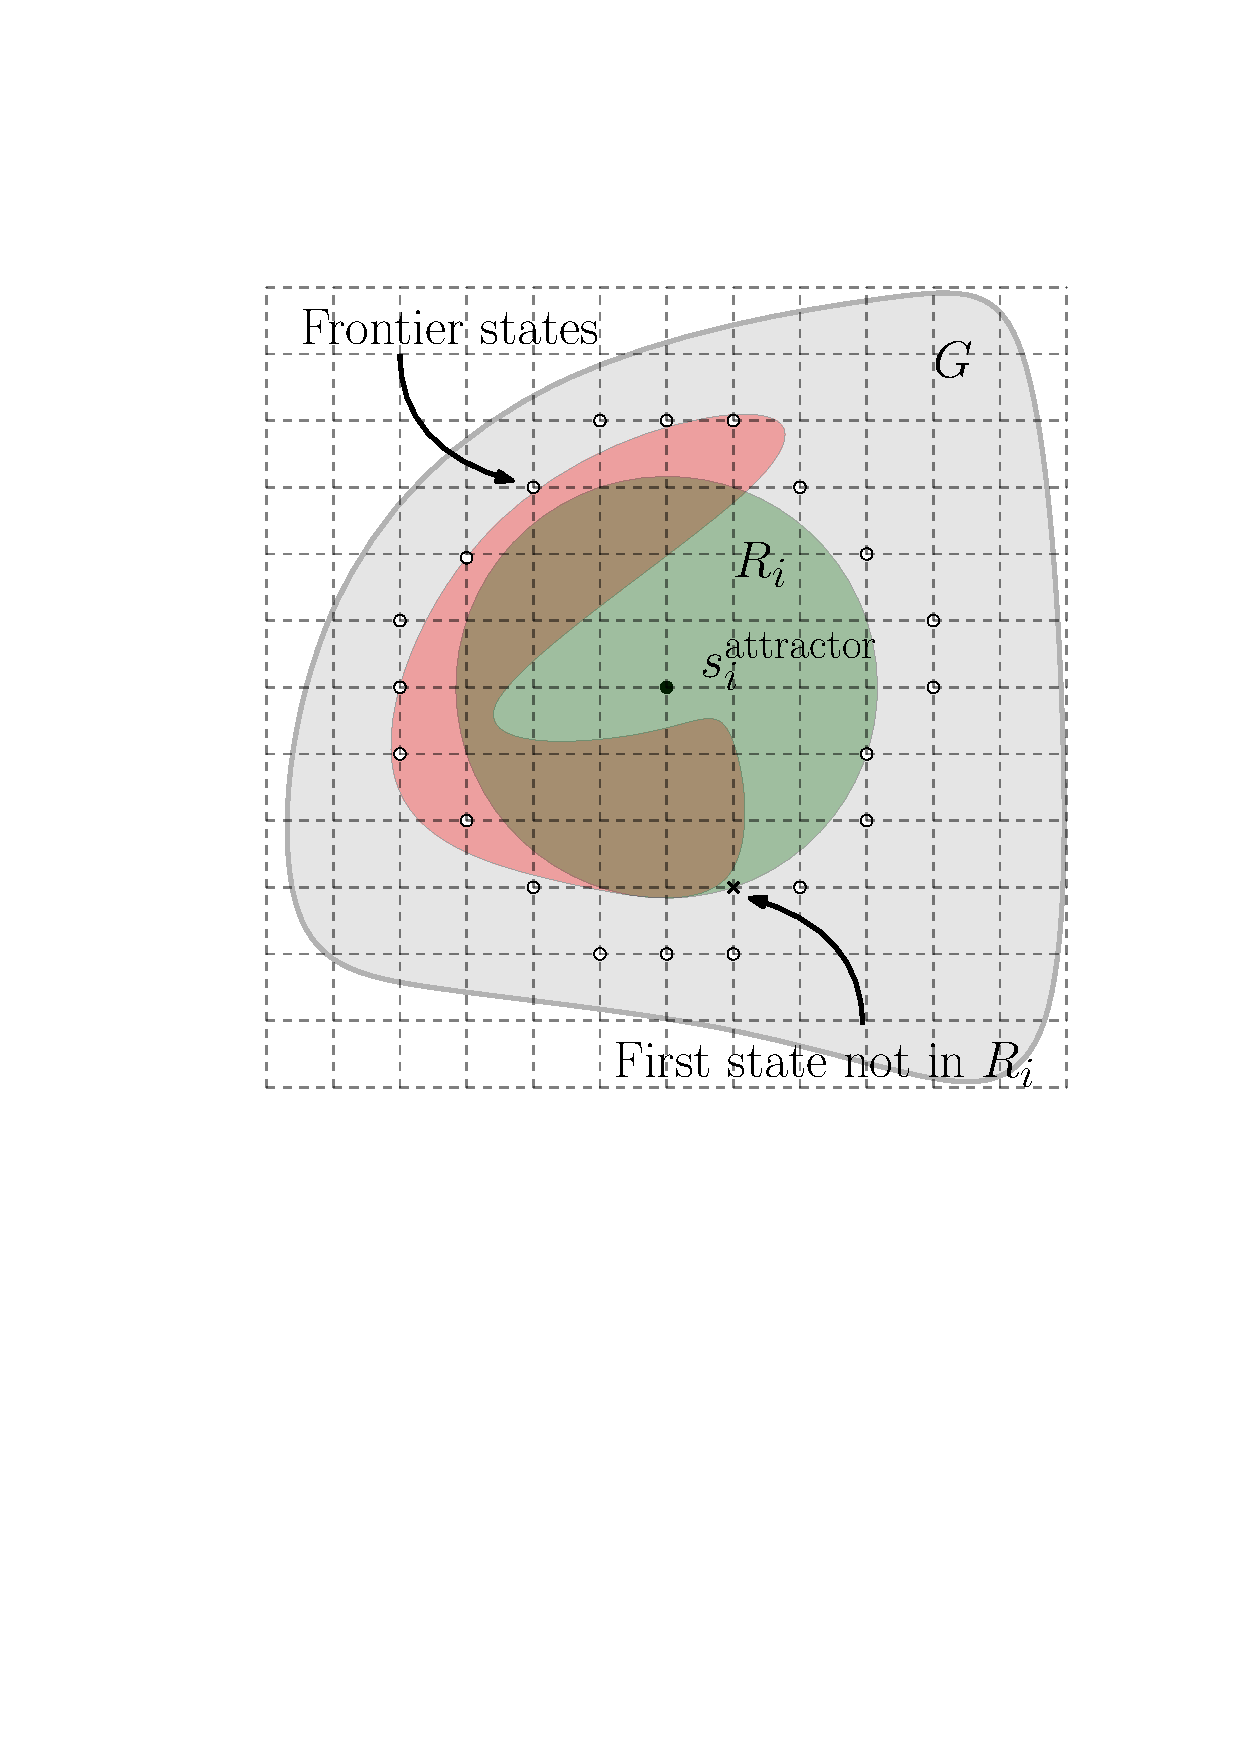
\includegraphics[width=0.20\textwidth]{Alg2.pdf}
  	% \vspace{-2mm}
  \caption{
  Visualization of Alg~\ref{alg:2}. Subregion $R_i$ (green) grown from $\sAttract$ in a goal region~$G_\calS$ (grey) containing an obstacle (red).
  Frontier states  and first state not in $R_i$ are depicted by circles and a cross, respectively.
}
   	\label{fig:alg2}
 \vspace{-6mm}
\end{figure}


% 1865 regions 984 secs

\paragraph*{Reachability Search}
The core of our planner lies in the way we compute the subregions (Alg.~\ref{alg:2} and Fig.~\ref{fig:alg2}) which we call a ``Reachability Search''. The algorithm maintains a set of \emph{reachable} states $S_{\text{reachable}}$ for which property P1 holds. 
Namely, the greedy successor\footnote{A state $s' \in \text{Succ}(s)$ is said to be a \emph{greedy} successor according to some heuristic $h(\cdot)$ if it has the minimal $h$-value  among all successors.} $s'$ of every reachable state $s \in S_{\text{reachable}}$ is also a reachable state, except for the attractor state \sAttract. 
This will ensure that in the query phase, we can run a greedy search from any reachable state $s \in S_{\text{reachable}}$ and it will terminate in the attractor state. 

The algorithm computes a subregion that covers the maximum number of reachable states that can fit into a hyper-ball defined by $h(s,\sAttract)$. 
The search maintains a priority queue OPEN ordered according to $h(s,\sAttract)$. Initially, the predecessors of $\sAttract$ are inserted in the OPEN (line~\ref{alg:2:OPEN}). For each expanded predecessor, if its valid greedy successor is in $S_{\text{reachable}}$, then the predecessor is also labeled as reachable (lines~\ref{alg:2:crit} and~\ref{alg:2:set}). 
%As the priority used for OPEN is the heuristic function, the radius of this hyper-ball keeps on increasing (line~\ref{alg:2:rad}). 


The algorithm terminates when the search pops a state which is valid but does not have a greedy successor state in $S_{\text{reachable}}$ (line~\ref{alg:2:terminate}). Intuitively, this corresponds to the condition when the reachability search exists an obstacle (see Fig.~\ref{fig:alg2}). At termination, all the states within the boundary of radius $r_i$ (excluding the boundary) are reachable.


\begin{algorithm}[t]
\footnotesize
\caption{Reachability Search}\label{alg:2}

\begin{algorithmic}[1]
\Procedure{ComputeReachability}{$\sAttract$}
%\Procedure{ComputeReachability}{$\sAttract, r_{\text{max}}$}
\State $S_{\text{reachable}} \leftarrow \{\sAttract\}$ \Comment{Reachable set} \label{alg:2:reachable}
\State OPEN $\leftarrow \{$Preds($\sAttract$)$\}$  \Comment{key: $h(s,\sAttract)$} \label{alg:2:OPEN}
\State CLOSED $\leftarrow \emptyset$
\State $r_i \leftarrow 0$

%\While {$r_i \leq r_{\text{max}}$}
\Loop{}
    \State $s \leftarrow$ OPEN.pop()
    \State insert $s$ in CLOSED
    \State $s'_g \leftarrow \arg \min_{s' \in \text{Succ}(s)} h(s', \sAttract)$ 
%    \State $s'_g \leftarrow$ GreedySucc($s$) 
 \Comment{greedy succesor}
 % acc. to some tie-breaking criteria}
    \If {$s'_g$ $\in$ $S_{\text{reachable}}$ and Valid(edge(s,$s'_g$))}  \label{alg:2:crit}
        \State $S_{\text{reachable}} \leftarrow S_{\text{reachable}} \cup \{s\}$  \Comment{$s$ is greedy} \label{alg:2:set}
    \ElsIf {Valid($s$)} \label{alg:2:terminate}
		\State \Return $r_i$
%        \State break
    \EndIf
    \State $r_i \leftarrow h(s, \sAttract)$ \label{alg:2:rad}
    \For {each $p \in \text{Preds}(s)$}
        \If {$p \notin$ CLOSED}
            \State insert $p$ in OPEN with priority $h(p, \sAttract)$
        \EndIf
    \EndFor
\EndLoop
%\EndWhile
%\State \Return $r_i$

\EndProcedure
\end{algorithmic}
\end{algorithm}

\subsubsection{Query Phase}
For any query goal state $s_{\text{goal}} \in G_\calS$, we find a subregion $R_i \in \calR$ which covers it. Namely, a region~$R_i$ for which 
$h(s_{\text{goal}}, \sAttract) < r_i$.
We then run a greedy search starting from $s_{\text{goal}}$ by iteratively finding for each state $s$ the successor with the minimum heuristic $h(s, \sAttract)$ value until the search reaches \sAttract. The traced path is then stitched to the corresponding precomputed path~$\pi_i \in \calL$. 
Note that at no point  do we need to perform collision checking in the query phase.

\begin{algorithm}[t]
\footnotesize
\caption{Query}\label{alg:3}

\begin{algorithmic}[1]
\Procedure{FindGreedyPath}{$s_1, s_2$}
	\State $s \leftarrow s_1$
	\While{$s \neq s_2$}
    	\State $s'_g \leftarrow \arg \min_{s' \in \text{Succ}(s)} h(s, s_2)$ 	\Comment{greedy succesor}
    	\State $s \leftarrow s'_g$
    	\State $\pi \cup \{s\}$ 
    \EndWhile
    \State \Return $\pi$
\EndProcedure

\Procedure{Query}{$\sGoal$}
	\For {each $R_i \in \calR$}
		\State $(\sAttract, r_i)$ $\leftarrow$ ${R_i}$;
		\If {$h(s_{\text{goal}}, \sAttract) < r_i$}
  		\State $\pi_g \leftarrow$ \textsc{FindGreedyPath} ($\sGoal, \sAttract$)
  		\State \Return $\pi_g \cup \pi_i$	\Comment{$\pi_i \in \calL$}
    \EndIf
	\EndFor
% \State $S_{\text{reachable}} \leftarrow \{\sAttract\}$ \Comment{Reachable set} \label{alg:2:reachable}
% \State OPEN $\leftarrow \{$Preds($\sAttract$)$\}$  \Comment{key: $h(s,\sAttract)$} \label{alg:2:OPEN}
% \State CLOSED $\leftarrow \emptyset$
% \State $r_i \leftarrow 0$

% %\While {$r_i \leq r_{\text{max}}$}
% \Loop{}
%     \State $s \leftarrow$ OPEN.pop()
%     \State insert $s$ in CLOSED
%     \State $s'_g \leftarrow \arg \min_{s' \in \text{Succ}(s)} h(s', \sAttract)$ 
% %    \State $s'_g \leftarrow$ GreedySucc($s$) 
%  \Comment{greedy succesor}
%  % acc. to some tie-breaking criteria}
%     \If {$s'_g$ $\in$ $S_{\text{reachable}}$ and Valid(edge(s,$s'_g$))}  \label{alg:2:crit}
%         \State $S_{\text{reachable}} \leftarrow S_{\text{reachable}} \cup \{s\}$  \Comment{$s$ is greedy} \label{alg:2:set}
%     \ElsIf {Valid($s$)} \label{alg:2:terminate}
% 		\State \Return $r_i$
% %        \State break
%     \EndIf
%     \State $r_i \leftarrow h(s, \sAttract)$ \label{alg:2:rad}
%     \For {each $p \in \text{Preds}(s)$}
%         \If {$p \notin$ CLOSED}
%             \State insert $p$ in OPEN with priority $h(p, \sAttract)$
%         \EndIf
%     \EndFor
% \EndLoop
%\EndWhile
%\State \Return $r_i$

\EndProcedure
\end{algorithmic}
\end{algorithm}


% which makes the query phase highly efficient.

\section {Analysis}

\begin{lemma}
\label{lemma:1}
A greedy search with respect to $h(s, \sAttract)$ starting from any reachable state $s$ $\in$ $R_i \cap G_\calS$ towards the corresponding attractor state $\sAttract$ is complete.
\end{lemma}

\begin{proof}
We can prove this lemma by contradiction. Firstly the greedy search in the query phase will always expand states which are $reachable$ because the greedy successor of every reachable state is also reachable (This is by the construction of Alg.~\ref{alg:2}). If we show that the greedy search will not encounter any cycles or in other words it will never reexpand a state, we prove that the search will eventually reach $\sAttract$ and is hence complete.


For the greedy search to get stuck in a cycle, the greedy successor of every state in the loop must also be a part of the loop, or in other words there cannot exist a state in the loop with its greedy successor exiting the loop. But that is not possible since at least the first state in this loop that got added to $S_{\text{reachable}}$ must have a greedy successor from outside the loop and must also belong to $S_{\text{reachable}}$ with a valid edge connecting to it (Alg.~\ref{alg:2}, lines~\ref{alg:2:crit} and~\ref{alg:2:set}). Hence the theorem is proved.
\end{proof}

\begin{lemma}
\label{lemma:2}
For any subregion $R_i \in \calR$, every state $s$ with $h(s,\sAttract) < r_i$ is reachable.
\end{lemma}

\begin{proof}
We will again prove this lemma by contradiction. Assume that there exists a state $s$ with $h(s,\sAttract) < r_i$ and was still not marked as $reachable$ in the reachability search. In that case along the path from $s$ to $\sAttract$, traced by the greedy search there must exist at least one state $s'$ s.t. $h(s',\sAttract) > r_i$. The reason is that as the reachability search expands states in the order of minimum heuristic value, $s'$ will never get expanded and thus will block the search from covering $s$. But since we assume that the heuristic function is weekly monotonic, this hypothesis cannot be true and hence there cannot exist such a state $s$.
\end{proof}

\begin{theorem}
For any goal state $s_{\text{goal}} \in R_i \cap G_\calS$ (i.e $h(\sGoal,\sAttract) < r_i$), a greedy search with respect to $h(s, \sAttract)$ over $\calS$ starting at $\sGoal$ will result in a collision-free path to \sAttract. 
\end{theorem}

\begin{proof}
The proof directly follows from the two lemmas. If for any goal state $\sGoal$, $h(\sGoal,\sAttract) < r_i$, then $\sGoal$ is reachable (Lemma~\ref{lemma:1}) and the greedy search towards $\sAttract$ is complete (Lemma~\ref{lemma:2}). Also as Alg.~\ref{alg:2} ensures that the transitions to the greedy successors are always valid we can guarantee that the greedy search will always return a valid path from $\sGoal$ to $\sAttract$.
\end{proof}

\begin{lemma}
Alg. ~\ref{alg:2} returns the maximum radius $r_i$ for a subregion $R_i$ within which every state $s$ with $h(s,\sAttract) < r$ is reachable. 
\end{lemma}

\begin{proof}
{\color{blue} May be it is obvious and should just be added as a note and not a theorem.}
% Once again we will prove by contradiction. Say Alg.~\ref{alg:2} returns a radius $r_{\text{max}} > r_i$. In that case the popped state $s$ for which Alg.~\ref{alg:2} terminated for not having a valid transition to a greedy successor which is also $reachable$ (lines~\ref{alg:2:crit} and~\ref{alg:2:set}), will also be included in $R_i$ while indeed it is not reachable. 
\end{proof} 

\subsection{Time Complexity of Query Phase}
The query time comprises of 
(i)~finding the containing subregion $R_i$ 
and
(ii)~running the greedy search to $\sAttract$.
Step (i) requires iterating over all subregions (in the worst case) which takes $O(|\calR|)$ steps while 
step (ii) requires expanding the states along the path from $\sGoal$ to $\sAttract$ which requires $O(\calD)$ expansions where $\calD$ is the depth of the deepest subregion. We can measure the depth of each subregion in Alg.~\ref{alg:2} by keeping track of the depth of each expanded state from the root i.e. the $\sAttract$. Hence, overall the query phases takes $O(|\calR| + \calD)$ operations. The maximal query time can also be empirically computed after the preprocessing phase.

%
Note that we can also bound the number of expansions required for the query phase by bounding the maximum depth of the subregions. We can do that by terminating Alg.~\ref{alg:2} when the $R_i$ reaches the maximum depth or if the existing termination condition (line ~\ref{alg:2:terminate}) is satisfied.

\section{Evaluation}
\begin{table}[tb]
  % \begin{center}
    \resizebox{\linewidth}{!}{%
      \begin{tabular}{ l | c c c c}
         & \textsf{PRM} (T) & \textsf{PRM} (2T) & \textsf{PRM} (4T) & Our method \\
       \hline
       Planning time [ms]& 20.2 (28.2) & 21.8 (34.1) & 22.9 (31.9) & 0.48 (1.01)\\
       % Planning time [ms]& 6.8 (12.2) & 7.2 (18.0) & - (-) & 0.48 (1.01)\\
       Success rate [$\%$] & 92 & 97 & 100 & 100 \\
       % Success rate [$\%$] & 90 & - & - & 100 \\
      \end{tabular}
  }
    \caption{Experimental results comparing our method with \textsf{PRM}. The table shows the mean/worst-case planning times and success rates for our method and for \textsf{PRM} preprocessed with equal, double and quadruple the time that our method takes in precomputation (T = 984 seconds).}
    \label{tab:stats}
  % \end{center}
 \vspace{-6mm}
\end{table}

We evaluated our algorithm by getting some preliminary results on the PR2 robot for the single-arm (7 DOF) planning problem. The task here is to repeatedly pick up objects from a conveyor belt and put them in a bin. 
We define the task-relevant goal region~$G$ by bounding the position and orientation of the end effector. 

%As mentioned, our method allows to guarantee bounds on the query time. The worst-case query time is bounded using the radius of the largest subregion and the total number of subregions that cover $G$. 
%After the preprocessing stage we can compute it by adding the lookup time for iterating over all the regions, and the time that the greedy search takes to reach the attractor from a goal state lying on the boundary of the largest subregion.

%\subsection{Results}
We compared our approach with the \textsf{PRM} algorithm in terms of success rate and planning times (see Table~\ref{tab:stats}) for 100 uniformly sampled goal states from $G$. 
Preprocessing (Alg.~\ref{alg:1}) took 984 seconds and returned 1,865 subregions. For a fair comparision, for \textsf{PRM} the paths from all the nodes in~$G$ to $s_{\text{start}}$ were precomputed. 
In the query phase if \textsf{PRM}'s connect operation fails for a given query, we consider it a failure. 
We also bootstrap \textsf{PRM} with 20 goal states from~$G$. Note that the worst-case time for our method shown in these results ($\sim$1 millisecond) is the empirical one and not the computed provable time bound which is 4 milliseconds for this environment.
 % \vspace{-5mm}

 \section{Conclusion}
We proposed a preprocessing-based motion planning algorithm that provides provable real-time performance guarantees for repetitive tasks and showed preliminary results. We aim to perform experiments on the hardware with the conveyor setup to demonstrate the efficiency of our planner on a real world system. Moreover on the theoretical side, we aim to provide guarantees on the solution quality.

% \begin{figure}[tb]
%   \centering
%     \includegraphics[width=0.20\textwidth]{simulation3.png}
%     % \vspace{-2mm}
%   \caption{
%   Experimental setup---The grid (in blue) depict the 3D projection of the goal region $G_\calS$.
% }
%     \label{fig:sim}
%  \vspace{-8mm}
% \end{figure}



%\section{Conclusion}
%Proofs
%
%Computational complexity

%%%%%%%%%%%%%%%%%%%%%%%%%%%%%%%%%%%%%%%%%%%%%%%%%%%%%%%%%%%%%%%%%%%%%%%%%%%%%%%%
\bibliographystyle{aaai}
\bibliography{references}

\end{document}
